\documentclass[11pt]{report}

\usepackage[utf8]{inputenc}
\usepackage{algorithm}
\usepackage{algpseudocode}
\usepackage{hyperref}
\usepackage{graphicx}
\usepackage{subcaption}
\usepackage{booktabs}
\usepackage[square,sort,comma,numbers]{natbib}
\bibliographystyle{abbrv}
\usepackage{caption}
\captionsetup{font=footnotesize}
\captionsetup[sub]{font=footnotesize}

% Title Page
\title{\textbf{A Neural Network to solve square jigsaw puzzles}}
\author{Advanced Machine Learning \\ \\
  Project Report by \\
  Dominique Cheray and Manuel Krämer}

\begin{document}
\maketitle

\tableofcontents

\chapter{Introduction}
\subsubsection*{by Dominique Cheray}
Solving jigsaw puzzles is a pastime that children all over the world know well.
Given a set of often oddly shaped interlocking pieces with small parts of a
picture on top of them the goal is to assemble the pieces in the correct way to
reconstruct the full image. But solving puzzles is not only a fun pastime it
also finds its applications in areas such as archaeology \cite{brown2008system,
  liu2011automated, koller2006computer}, biology
\cite{marande2007mitochondrial}, speech descrambling \cite{zhao2007puzzle},
image editing \cite{cho2008patch} or the reconstruction of fragmented documents
\cite{zhu2008globally}.

The first automatic jigsaw puzzle solvers focus only on the shape of the pieces
to solve the puzzles \cite{freeman1964apictorial, wolfson1988solving,
webster1990computer, kong2001solving}. Later on approaches are presented, which
take into account the color information in addition to the shape of the pieces
\cite{kosiba1994automatic, makridis2006new, sagiroglu2006texture}. Recent work
began to focus on only using the color information of the pieces
\cite{nielsen2008solving} which then eventually shifted to only consider jigsaw
puzzles with square pieces where color information is the only information that
can be used to find matching pieces \cite{Cho2010, yang2011particle,
  Pomeranz2011, gallagher2012jigsaw, son2014solving, sholomon2013genetic,
  Paikin2015, sholomon2016dnn}.

The first to introduce square pieces are Cho et al. \cite{Cho2010}. They present
a probabilistic solver that can handle puzzles of up to 432 pieces. To solve the
puzzle the solver needs some apriori knowledge of the puzzle, namely its size
and the position of few so-called ``anchor-pieces'' which are placed at their
correct location prior to the placement of the remaining pieces. A year later
the results of Cho et al. are improved by Yang et al. \cite{yang2011particle}
which use a particle filter based solver.

Pomeranz et al.\cite{Pomeranz2011} are the first to introduce a fully automatic
jigsaw puzzle solver. Their solver is based on a greedy placer and can handle
puzzles of up to 3,300 pieces. Later on the work of Pomeranz et al. is improved
and extended by both Gallagher et al. \cite{gallagher2012jigsaw} and Son et al.
\cite{son2014solving}. Gallagher use a greedy tree algorithm and generalize the
work of Pomeranz et al. to also handle pieces of unknown orientation and puzzles
with unknown dimensions. Son et al. add ``loop constraints'' to the work of
Gallagher et al. which allows them to handle pieces of unknown orientation.

Instead of a greedy solver Sholomon et al. \cite{sholomon2013genetic} present a
genetic algorithm that is able to solve large square jigsaw puzzles. Later on
they improve their work by introducing a deep neural-network based estimation
metric \cite{sholomon2016dnn}. Given the edges of two pieces the neural network
predicts whether the two pieces belong next to each other in the correctly
assembled puzzle or not. The authors state that their metric shows
extremely high precision without the need of manual feature extraction. When
integrated into an existing solver it will significantly improve the results
\cite{sholomon2016dnn}. 

The solver presented by Paikin \& Tal \cite{Paikin2015} is inspired by the work
of Pomeranz et al. \cite{Pomeranz2011}. Their algorithm is also a greedy solver
but is able to solve more challenging puzzles. It can handle jigsaw puzzles with
missing pieces, pieces of unknown orientation, puzzles of unknown size and
multiple puzzles whose pieces are mixed together. The placement of the puzzle
pieces is based on a compatibility function but they provide a faster and more
accurate function than previous works. Additionally, since early mistakes can
have a fatal impact when using a greedy placer, they take special care when
choosing the first piece to place. Earlier works randomly select the first
piece. Another change made by Paikin \& Tal is to place the pieces in relation
to the pieces already placed and not on absolute positions. So the next piece to
place is not the piece that best fits a particular spot, but the most likely to
be correct.

For this project we will integrate the neural-network based estimation metric
proposed by Sholomon et al. \cite{sholomon2016dnn} in our reimplementation of the
solver by Paikin \& Tal \cite{Paikin2015} from last semester's project. We evaluate the resulting
solver with the same image datasets as the authors and compare our result to
theirs as well as to the results from our implementation of Paikin \& Tal's
solver from last semester.

\chapter{Theoretical Background}
\subsubsection*{by Dominique Cheray}
\section{Automatic Jigsaw Puzzle Solvers}
The first jigsaw puzzles were made out of wood and produced around 1760 by John
Spilsbury a London engraver and mapmaker. The name ``jigsaw'' refers to the
jigsaws that were used to cut out the pieces of the puzzles. Modern jigsaw
puzzles made out of cardboard sheets with an image printed on top and cut into a
set of interlocking pieces were introduced in the 1930s
\cite{williams2004jigsaw}. Even though children worldwide solve puzzles
successfully, automatic puzzle solvers are a technically challenging problem.
Demaine et al. \cite{demaine2007jigsaw} show that, if the pairwise affinity
among pieces is unreliable, the puzzle problem is NP-complete.

In 1964 Freeman et al. \cite{freeman1964apictorial} propose the first automatic
jigsaw puzzle solver. It can handle puzzles of up to nine pieces which are all
uniformly gray and the only available information being the shape of the pieces.
Various other early works use aspects piece shape information or contour
matching to solve jigsaw puzzles. Wolfson et al. \cite{wolfson1988solving}, for example first
reconstruct the boundary of the jigsaw puzzle and then gradually fill the inside
with the most reliably matching piece. An approach which is also widely used by
humans. Webster et al. \cite{webster1990computer} introduce a methodology
based on a so called Isthmus. An Isthmus is a feature defined by a set of
critical points and can be used in matching boundaries of planar regions. Kong
et al. \cite{kong2001solving} present a two step approach. The first step
consists of using local shape matching to find likely candidate pairs for
adjacent fragments. The second step then resolves ambiguities that result from the
local shape matching by finding a global solution and finally the pieces are
merged together. They report successfully using their approach to reassemble
broken ceramic tiles and a map puzzle.

Kosiba et al. \cite{kosiba1994automatic} are the first to consider the color
information of a piece in addition to its shape. Depending on whether the
original image is known or not the color information is used differently. 
If the original image is known the overall color characteristic of each piece,
meaning the mean and variance of the hue, saturation and intensity values, are
calculated. These features are then compared with color characteristics of
various regions in the original image to try to reassemble the jigsaw puzzle in
the same orientation as the original image. If the original image is unknown
small color windows at regular intervals along the borders of the pieces are sampled
and color characteristics for each of these windows are calculated. These
features, together with the shape information of the pieces, are then used to
compare the borders of pieces and find likely matching pairs. Makridis et al.
\cite{makridis2006new} consider a puzzle as an image composed of a number of
subimages (pieces). In their approach a set of boundary characteristics points and for each
characteristic point a set of color and geometrical features are extracted for
each pieces. To decide whether two subimages match or not the sets of features
are compared. When two pieces are considered matching pieces they are
merged together to form a new subimage. The algorithm then proceeds with the new
subimage and the remaining subimage until either all subimages were merged to
one final image or no more matching subimages can be found. Sagiroglu et al.
\cite{sagiroglu2006texture} use textural features and geometrical constraints
instead of color information to find matching pieces. Their texture prediction
algorithm predicts pixel values in a band outside the border of the piece. The
original pictorial specifications of possible neighboring pieces are then
compared to the textural features of this predicted band to find a matching
pair. The aim is to maximize the matching continuity of the texture while
satisfying the geometrical constraints.

The first to disregard the shape information entirely and only use the image
features to solve a jigsaw puzzle are Nielsen et al. \cite{nielsen2008solving}.
They only look at a single-pixel wide continuous strip for each edge of a piece.
If there is little to no gradient at the common edges of two pieces they are
considered a likely match. Using this approach they are able to not only solve
jigsaw puzzles with many similar or identical shaped pieces, but also jigsaw
puzzles consisting of only rectangular pieces. Cho et al. \cite{Cho2010} take
this one step further and look exclusively at puzzles that consist of only
square pieces. They develop a graphical model to solve the jigsaw puzzles. In
their approach a set of ``anchor pieces'' are fixed at the correct location
before placing of the remaining pieces starts. To solve puzzles of over 400
pieces only 4 to 6 pieces need to be fixed at their correct location. They also
introduce a dissimilarity based compatibility function to quantify the pairwise
distance between two pieces which became the basis of most future work. The
sum-of-squared color differences along the abutting boundary is calculated to
determine how similar two pieces are. The results of Cho et al. are later on
improved by Yang et al.\cite{yang2011particle} by using a particle filter.
Additionally the do not assume any prior knowledge of the image layout or
beforehand correctly placed pieces.

The first fully automatic square jigsaw puzzle solver is proposed by Pomeranz et
al. \cite{Pomeranz2011} and is based on a greedy placer and a novel prediction
based dissimilarity. Like Yang et al. \cite{yang2011particle} their solver does
not require prior knowledge about the image or previously correctly placed
pieces. Only the pieces themselves, their orientation and the dimensions of the
puzzle are given as input to the solver. The jigsaw puzzle is then solved by the
greedy solver in several steps. First, to measure the affinity between the
pieces the compatibility function is calculated. Second, the placement is
executed. Given a single pieces or a partially constructed puzzle, the placer
tries to find the position of the remaining parts on the board. Next step is a
segmentation step. A partial solution from the previous step, meaning the
placement of all pieces on the board, is divided into segments which are
estimated to be assembled correctly, disregarding their absolute location. In a
fourth step shifting is performed, meaning that given a set of puzzle segments
these segments and remaining individual pieces are relocated on the board to
obtain a better approximate solution. All these steps are then repeated until
evaluation of the best buddies metric reaches a local maximum. The best buddies
metric is a metric to determine how likely neighboring pieces are true
neighbors. Gallagher et al. \cite{gallagher2012jigsaw} introduce a greedy tree
algorithm to also solve square jigsaw puzzles whose dimensions are not known and handle pieces
of unknown orientation. Additionally their jigsaw piece compatibility measure is
Mahalanobis inspired. Their approach is extended by Son et al.
\cite{son2014solving} who add loop constraints. They use a loop-based strategy
to reconstruct jigsaw puzzles from the local matching candidates. Their
algorithm seeks out and exploits loops as a form of outlier detection.

Sholomon et al. \cite{sholomon2013genetic} refrain from the use of a greedy
solver but introduce a genetic algorithm as a strategy for piece placement. The
placements of all puzzle pieces are the population of chromosomes a genetic
algorithm contains. They start with 1,000 chromosomes meaning 1,000 random
placements. A fitness function based on the pairwise compatibility of every pair
of adjacent pieces is used to evaluate the population at each generation. A new
population is produced by selection of chromosomes and the crossover of
chromosome pairs. The probability of a chromosome to be chosen for either
crossover or directly becoming part of the next generation is directly
proportional to the value of its fitness function. Later on Sholomon et al.
introduce a neural network-based estimation metric to solve square jigsaw
puzzles \cite{sholomon2016dnn}. They train a neural network to predict, given
two puzzle piece edges, if those two pieces should be adjacent or not in the
correctly solved puzzle. If two piece edges are considered to be neighbors by
the neural network they are called \textit{DNN-Buddies}. This \textit{DNN-Buddy}
metric is incorporated in the following way into the genetic algorithm of
Sholomon et al.: Whenever a \textit{DNN-Buddy} pair is present in one of the
parents this pair is assigned in the child. A more detailed description of the
neural network and its training will follow in the next chapter in which we
elaborate on how we integrated the \textit{DNN-Buddy} metric into our
implementation of the puzzle solver proposed by Paikin \& Tal \cite{Paikin2015}.

Paikin \& Tal \cite{Paikin2015} propose an approach that is inspired by Pomeranz
et al. \cite{Pomeranz2011}. They also use a greedy solver and the placement of
the pieces is based on the compatibility between pieces. But their proposed
compatibility function is more accurate and faster than previous compatibility
functions. It not only takes advantage of the similarity between pieces but also
considers the reliability of this similarity. Additionally they take special
care when selecting the first piece to place since a greedy algorithm is
extremely vulnerable to early errors. Paikin \& Tal require the first piece to
have distinctive borders and lie in a distinctive region. This is in contrast to
earlier works, in which the first piece is randomly selected. Furthermore, they
do not chose the best piece for a specific location, but the piece that
minimizes the likelihood of making a mistake, regardless of its position. This
approach allows them to solve jigsaw puzzles with additional challenges like
puzzles with missing pieces, puzzles of unknown size, puzzles with pieces whose
orientation is unknown and multiple puzzles whose pieces are mixed together. For
the multiple puzzles problem there is no information about the sizes of the
puzzles or possibly missing pieces needed. Only the number of puzzles to solve
is known. A more detailed description of the solver by Paikin \& Tal will be
provided in the following chapter in which we elaborate on our implementation of
the solver and the integration of the \textit{DNN-Buddy} metric into it. 

\chapter{Materials and Methods}
\subsubsection*{by Manuel Krämer}
\section{Algorithm}
\label{sec:algo}
The algorithm we implemented is the one that was used in \cite{Paikin2015} with the extension of a neural network as proposed by \cite{sholomon2016dnn}. The whole procedure can be described by three main steps:
\begin{enumerate}
	\item Compatibility between pieces: This is done by calculating the dissimilarity between two pieces. The so-called "Best Buddies"-metric, which was used by \cite{Paikin2015}, is replaced by the DNN-Buddies that are determined by a Neural Network. This metric indicates, that two pieces agree that each other is their best neighbor.
	\item First piece: As described by \cite{Paikin2015} one important step is to find a good starting piece which has best buddies in all four spatial relations and these four neighbors have best buddies in all directions as well.
	\item Placer: The placing of the pieces is done by grabbing the best piece (highest compatibility) from a pool, placing this piece and adding the best buddies of it to the pool.
\end{enumerate}

\subsection{Compatibility between pieces}
The most fundamental part is the calculation of the compatibility between two pieces to determine how well they fit together. This is done by computing the dissimilarity between every pair of pieces and with this score you can tell if the pieces have similarities or not.

First of all, the dissimilarity of two pieces $p_i$ and $p_j$ is defined as follows (see \cite{sholomon2016dnn}): 
\begin{equation}\label{eq:dissimilarity}
	D(x_i,x_j,right) = \sqrt{\sum_{k=1}^K \sum_{d=1}^3 (p_i(k,K,cb) - p_j(k,1,cb))^2}
\end{equation}
K is the piece size and cb the color band.

\subsection{First piece}
One important task is to avoid early errors because the algorithm considers the unplaced and placed pieces as well. If there is a mistake within the first few pieces this can lead to following errors.
This means we need a first piece that is located in a distinctive area where the probability of making errors is as low as possible. A good measure for this is the DNN-buddies metric. We require the first piece to have best buddies in all four spatial relations, what ensures that the piece itself is distinctive. Furthermore, all four neighbors of this piece need to have best buddies in all four spatial relations as well, what means that the piece is located in a distinctive region. 
Usually, there is more than one piece that satisfies these conditions. Out of all these distinctive pieces we choose the one with the best buddies that maximize the compatibility in all four spatial relations.

\subsection{Placer}
The placer algorithm as described in \cite{Paikin2015} places all pieces according to their compatibility and maintains a pool with potential pieces to place. Since the description is not detailed there are several possibilities to implement it so we want to give a more comprehensive explanation of our method (see algorithm \ref{algo:placer}).

\begin{algorithm}
	\caption{Placer algorithm}
	\label{algo:placer}
	\begin{algorithmic}
		\State Place the first piece into the pool
		\While{There are unplaced pieces}
		\While{Pool is not empty}
		\State Get the best item and its placing position from the pool
		\If{Placing position is occupied}
		\State Delete the piece from processedPieces and continue \EndIf
		\State Add this item to the placer List
		\State Delete this item from unplaced pieces
		\State Save the taken indices
		\State Calculate all best buddies and put them in the pool
		\EndWhile
		\Comment{Pool is empty}
		\State Get best piece of all unplaced
		\If{Placing position is not occupied}
		\State Put this piece on the pool
		\EndIf
		\EndWhile
	\end{algorithmic}
\end{algorithm}

With this approach, we make sure that an already placed piece doesn't get overwritten by pieces that maybe have a high compatibility as well. While processing through all pieces we keep track of the row and column indices of every piece so we can detect duplicates and, finally reconstruct the puzzled image.
\newpage

\section{Neural Net}
The architecture of the neural net is the one proposed by \cite{sholomon2016dnn}. In Figure \ref{fig:NN} one can see that it is a simple 4-layer, fully-connected network which uses the two edge rows/columns of two adjacent pieces as an input. The classification between "best buddy" and "not best buddy" is done by a softmax classifier that produces the probability of the two cases. The activation for all layers is the rectified linear unit (ReLU) function and we trained the network with the Stochastic Gradient Descent.
\begin{figure}[ht]
	\centering
	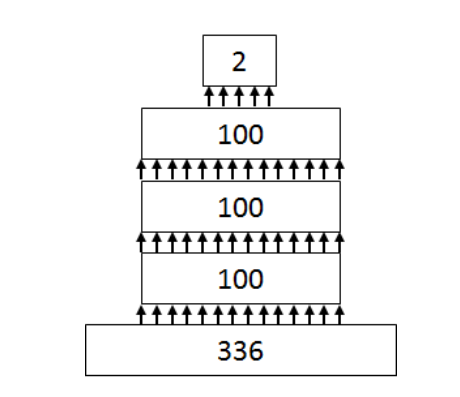
\includegraphics[width=0.6\textwidth]{NeuralNet.PNG}
	
	\caption{The architecture of the neural net (from \cite{sholomon2016dnn})}
	\label{fig:NN}
\end{figure}


\section{Image data and evaluation}
\subsection{Training data of the Neural Net}
For training and cross-validation we use 2218 images from the IAPR TC-12 Benchmark (see \cite{grubinger06}, one can see a sample of those in figure \ref{fig:IAPR-database}). These images have a resolution of 360 $\times$ 480 pixels and we convert them into YUV color space before processing. After normalization the images get cut into 12 $\times$ 17 tiles which are used to produce a training set for the neural network in the following way:
\begin{itemize}
	\item For each puzzle piece edge $x_{i,j}$, find the most compatible piece edge $x_{k1,l1}$ and its second most compatible piece edge $x_{k2,l2}$
	\item  If the pair $x_{i,j}$ - $x_{k1,l1}$ is originally adjacent, add this pair to the positive labeled and the pair $x_{i,j}$ - $x_{k2,l2}$ to the negative labeled
	\item If this is not the case, add $x_{i,j}$ - $x_{k1,l1}$ to the negative labeled and discard the pair $x_{i,j}$ - $x_{k2,l2}$
\end{itemize}
To decide if two pieces are adjacent the most important regions are the edges. So one (positive or negative) instance contains the two edge rows/columns of one piece and two adjacent rows/columns of the other. Since all images from \cite{grubinger06} have the same size the procedure described above results in an image array of 336 pixels (28 pixels $\times$ 4 rows/columns $\times$ 3 color chanels).

\begin{figure}
	\centering
	\begin{subfigure}[b]{0.45\textwidth}
		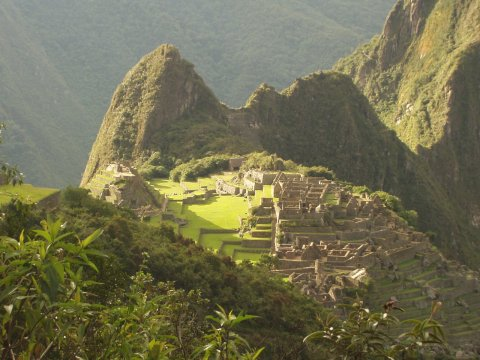
\includegraphics[width=\textwidth]{../iaprtc12/images/24/24019.jpg}
		\caption{One image of the dataset}
		\label{img1}
	\end{subfigure}
	~
	\begin{subfigure}[b]{0.45\textwidth}
		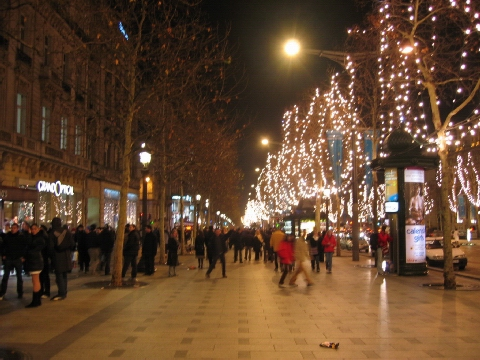
\includegraphics[width=\textwidth]{../iaprtc12/images/37/37142.jpg}
		\caption{Another image of the dataset}
		\label{img2}
	\end{subfigure}
	
	\caption{A sample of all the datasets we used for the training of the neural net}
	\label{fig:IAPR-database}
\end{figure}

\subsection{Evaluation}
By testing the algorithm we used images from \cite{Cho2010} (size: 432 pieces) and \cite{Pomeranz2011} (size: 540, 805 and 2360 pieces) to get comparable results. A small sample of these data one can see in fig. \ref{fig:database}

\begin{figure}
	\centering
	\begin{subfigure}[b]{0.45\textwidth}
		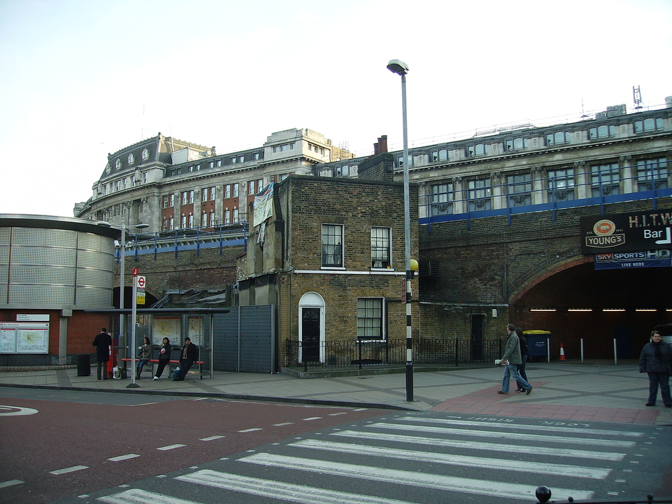
\includegraphics[width=\textwidth]{../imData/432/1.png}
		\caption{One image of the dataset we used for the puzzle with 432 pieces}
		\label{img:432}
	\end{subfigure}
	~
	\begin{subfigure}[b]{0.45\textwidth}
		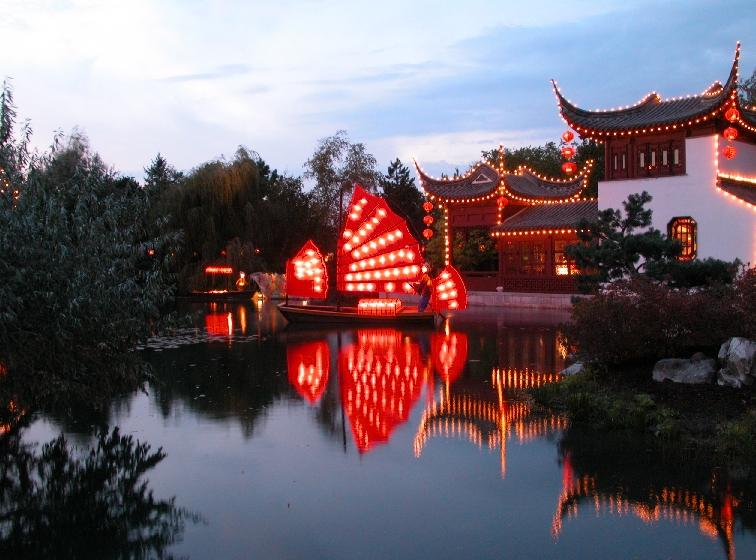
\includegraphics[width=\textwidth]{../imData/540/1.jpg}
		\caption{One image of the dataset we used for the puzzle with 504 pieces}
		\label{img:540}
	\end{subfigure}
	~
	\begin{subfigure}[b]{0.45\textwidth}
		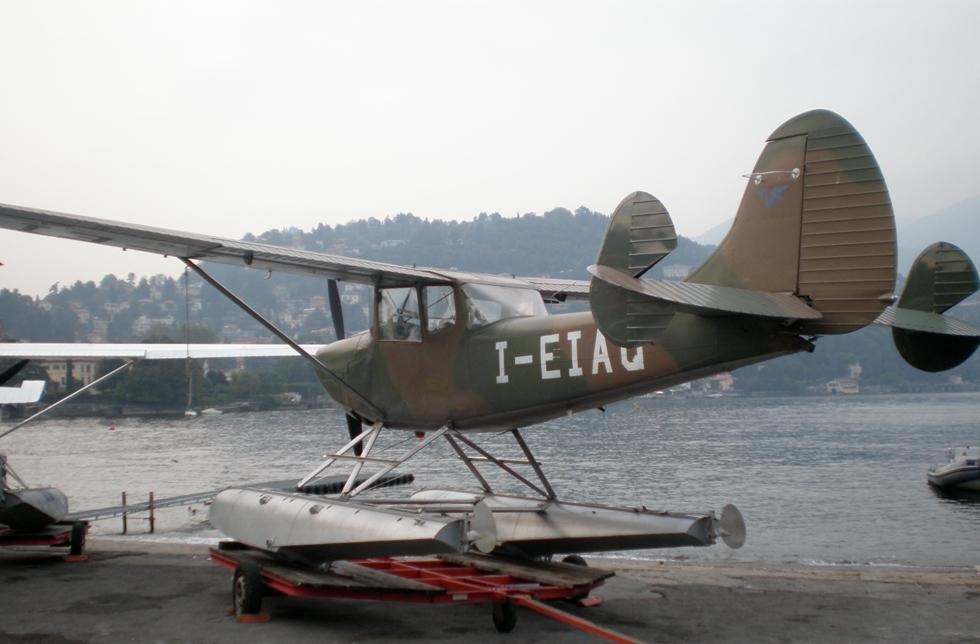
\includegraphics[width=\textwidth]{../imData/805/1.jpg}
		\caption{One image of the dataset we used for the puzzle with 805 pieces}
		\label{img:805}
	\end{subfigure}
	~
	\begin{subfigure}[b]{0.45\textwidth}
		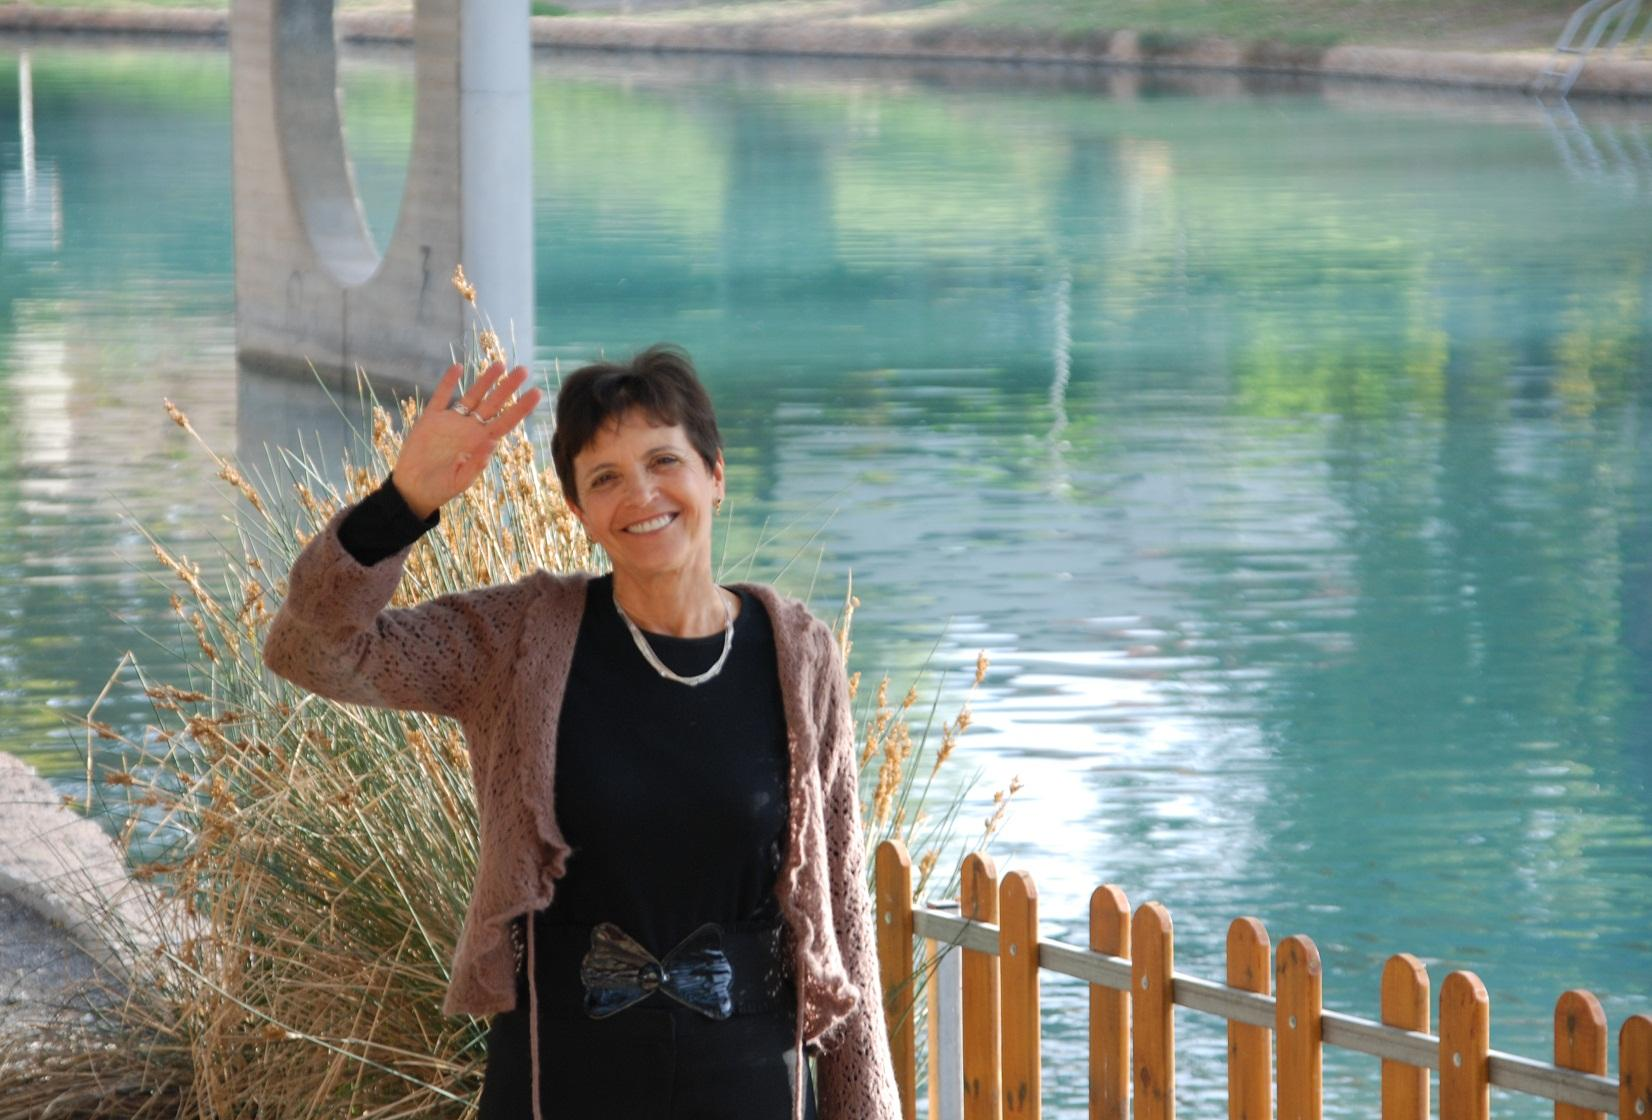
\includegraphics[width=\textwidth]{../imData/2360/1.jpg}
		\caption{One image of the dataset we used for the puzzle with 2360 pieces}
		\label{img:2360}
	\end{subfigure}
	
	\caption{A sample of all the datasets we used for evaluation}
	\label{fig:database}
\end{figure}

To evaluate our results we used the direct measure, i.e. to check the absolute position of every piece in the image and the relative score which determines how many correct neighbors each piece has.

\chapter{Results}
\subsubsection*{by Dominique Cheray}



We evaluate our implementation of the puzzle solver using the same image
datasets as Sholomon et al. \cite{sholomon2016dnn} and Paikin \&Tal
\cite{Paikin2015}. These are three sets of 20 images each. One set for 432-piece
puzzles, one set for 540-piece puzzles and one set for 805-piece puzzle. Also a
set of 3 images for 2360-piece puzzles. This set is only used by Paikin \& Tal
for the Evaluation. Sholomon et al. does not provide results for this dataset.
Furthermore, Paikin \& Tal test their solver on additional data sets for even
larger puzzles (up to 22,755 pieces). In the absence of the necessary hardware
required for the computational effort to solve these puzzles we are unable to
evaluate our implementation on these datasets.

We compare our results to those of Sholomon et al. \cite{sholomon2016dnn}, as
well as to those of Paikin \& Tal \cite{Paikin2015} since our solver is a fusion
of both approaches. We use the placer algorithm described by Paikin \& Tal but
extend it by the neural network-based estimation metric proposed by Sholomon et
al. Additionally we also consider the results of our reimplementation of Paikin
\& Tal's solver from last semester's project in order to provide insights in how
using the new estimation metric changed the results of the solver. Following the
above mentioned works, we apply our
solver to the classic puzzle problem, meaning there are no missing pieces or
mixed puzzles and the dimensions of the puzzle are known.

As a measure of accuracy we use the common absolute measure, that is the
proportion of pieces placed at their absolute correct location as well as the
neighbor measure, which considers the fraction of the correct pairwise
adjacencies. Additionally we report the number of puzzles that have been
reconstructed perfectly. Table \ref{resTable} shows the results, averaged for
the respective datasets.

\begin{table}[]
\caption{Comparison of our results to those of Sholomon et al.
    \cite{sholomon2016dnn}, those of Paikin \& Tal \cite{Paikin2015} and to
    those of our reimplementation of Paikin \& Tal's solver from last
    semester (Re \cite{Paikin2015}). '-' means the results are not reported.}
\label{resTable}
\resizebox{\textwidth}{!}{%
  \begin{tabular}{|c||c|c|c|c||c|c|c|c|
    |c|c|c|c|}
\hline
  & \multicolumn{4}{c||}{direct}                                                          & \multicolumn{4}{c||}{neighbor}                                                         & \multicolumn{4}{c|}{perfect}                                                       \\ \hline 
  \# of pieces & Our   & \cite{sholomon2016dnn} & \cite{Paikin2015} & Re \cite{Paikin2015} & Our    & \cite{sholomon2016dnn} & \cite{Paikin2015} & Re \cite{Paikin2015} & Our & \cite{sholomon2016dnn} & \cite{Paikin2015} & Re \cite{Paikin2015}
\\  \hline \hline
432         & 4.5\%  & -                      & 96.16\%            & 98.69\%                          & 59.22\% & 95.65\%                 & 95.82\%            & -                               & 0   & 12                     & 13                & 11                              \\ \hline
540         & 7.61\% & -                      & 93.22\%             & 88.21\%                          & 47.9\%  & 96.37\%                 & 96.1\%             & -                               & 0   & 11                     & 13                & 11                              \\ \hline
805         & 2.91\% & -                      & 92.47\%            & 91.72\%                          & 45.9\%  & 95.86\%                 & 95.09\%            & -                               & 0   & 8                      & 9                 & 7                               \\ \hline
2360        & 0.04\% & -                      & 94.01\%            & 88.13\%                          & 46.28\% & -                      & 96.26\%            & -                               & 0   & -                      & 1                 & 0                               \\ \hline \hline
Overall     & 3.77\% & -                      & 93.97\%            & 91.69\%                          & 49.58\% & 95.96\%                 & 95.82\%            & -                               & 0   & 31                     & 36                & 29                              \\ \hline
\end{tabular}%
}
\end{table}

For the 432-piece puzzles the fraction of correctly placed pieces does not in
the least reach the results of Paikin \& Tal not to mention the results of our
reimplementation. Although the proportion of correct neighbors  found by our
solver is significantly better than the direct measure it is still far from the
results of Sholomon et al. and Paikin \& Tal.
Not surprisingly, if one looks at the percentage of correctly placed pieces, we
can not perfectly reconstruct a single puzzle. Sholomon et al. perfectly
reconstruct 12 puzzles and Paikin \& Tal even 13. 

The direct measure for the 540-piece puzzles is slightly better than the one for
the 432-piece puzzles but still not at all comparable to those of Paikin \& Tal
or our reimplementation of their solver. The same applies to the correctly found
neighbors. We
do not even find half as many true neighbors as Sholomon et al. or Paikin \&
Tal. Again we can not perfectly reconstruct a single puzzle, while Sholomon et
al. achieve 11 perfectly reconstructed puzzles and Paikin \& Tal again 13. Only
our reimplementation of Paikin \& Tal's solver reaches the same number of
perfectly reconstructed puzzles as Sholomon et al.

Also for the 805-piece Puzzles, our results do not come close to those of
Sholomon et al, Paikin \& Tal or our reimplementation. Neither the direct
measure, nor the neighbor measure or the number of perfectly reconstruct
puzzles.

The proportion of correctly placed pieces for the 2360-piece puzzles is
negligible and in no way comparable to the results of Paikin \& Tal or our
reimplementation. Although we find much more correct neighbors than
correct placements of the pieces we are still far from the results of Paikin \&
Tal. Additionally they are able to perfectly reconstruct one puzzle, while we
again do not perfectly reconstruct a single one.

In summary, in none of the three metrics, direct metric, neighbor metric, number
of perfectly reconstructed puzzles do we even come close to the results of the
two solvers whose approaches we combine. Although our mere reimplementation of
Paikin \& Tal's solver from last semester showed results comparable to those of
Paikin \& Tal and even outperformed them in terms of direct measure for the
432-piece puzzles, the integration of the \textit{DNN-Buddy} metric proposed by
Sholomon et al. did not improve the solver. On the contrary, the solver shows
significantly worse results.

Figure \ref{fig:directMeasure} shows hows for each puzzle size we tested our
algorithm with the image that reaches the highest value in the direct metric.
Figure \ref{fig:neighborMeasure} shows the same for the neighbor metric. As one
can see, in almost all cases they are the same pictures. Only for the 432-piece
puzzle the image with the highest neighbor metric is a different one than the
one with the highest direct metric. In this picture one can clearly see a weak
point of the direct metric. The puzzle is solved almost perfectly, only the
bottom row of pieces has been misplaced on the top of the image. The direct
measure gives an accuracy of 0\% whereas the neighbor measure comes to a much
better result, namely 68.4\%. Since not finding a neighbor where a neighbor
should have been found, as it is the case if a non-border piece is placed at the
border, or finding a neighbor where no neighbor should have been,
as it is the case if a border piece is incorrectly placed in the inner part of
the image, this puzzle still only reaches 68.4\% although one would expect a
higher value at first.

\begin{figure}
	\centering
	\begin{subfigure}[b]{0.3\textwidth}
		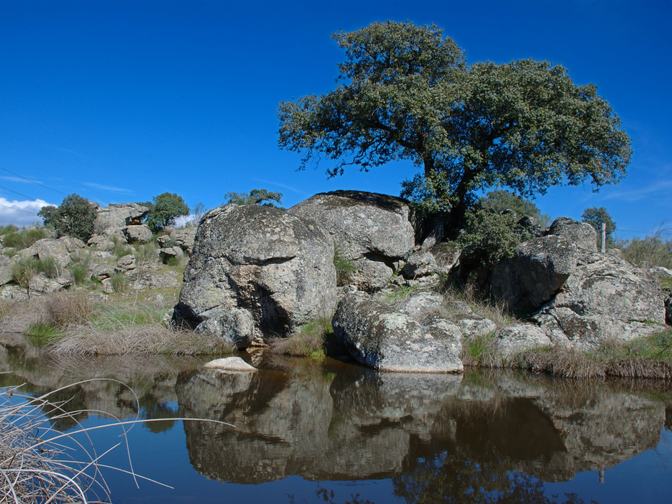
\includegraphics[width=\textwidth]{../imData/432/16.png}
		\caption{Original image}
	\end{subfigure}
	~
	\begin{subfigure}[b]{0.3\textwidth}
		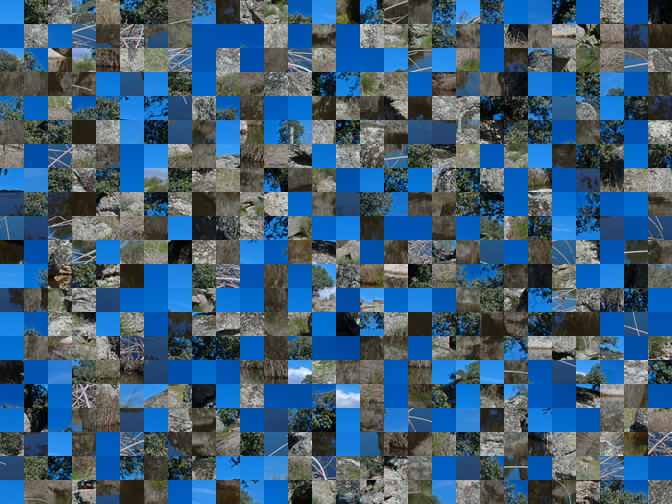
\includegraphics[width=\textwidth]{../results/432/16_shuffled.png}
		\caption{Shuffled image}
	\end{subfigure}
	~
	\begin{subfigure}[b]{0.3\textwidth}
		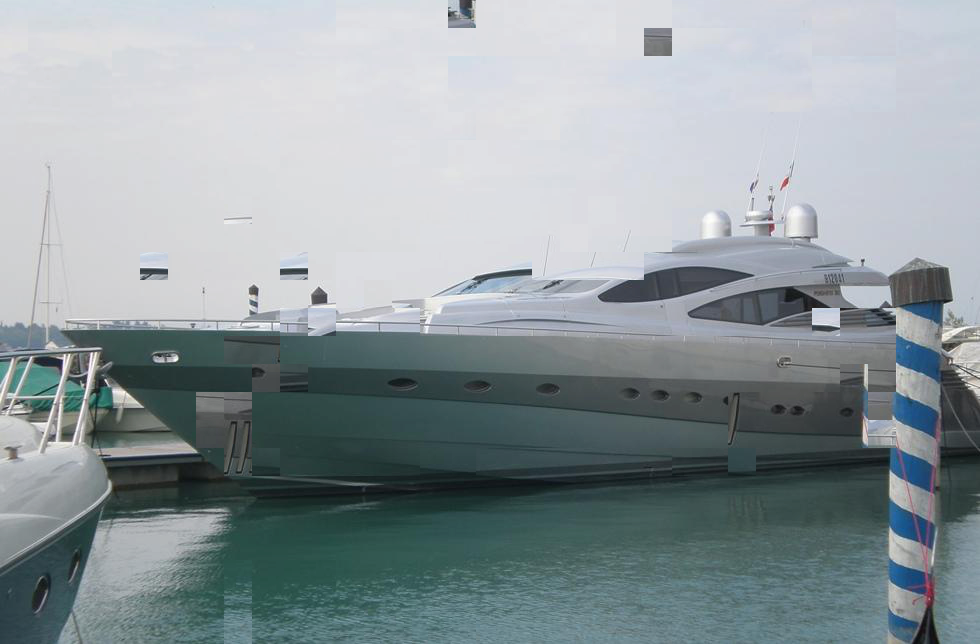
\includegraphics[width=\textwidth]{../results/432/16_solved.png}
		\caption{Solved image}
	\end{subfigure}
  ~
  \begin{subfigure}[b]{0.3\textwidth}
		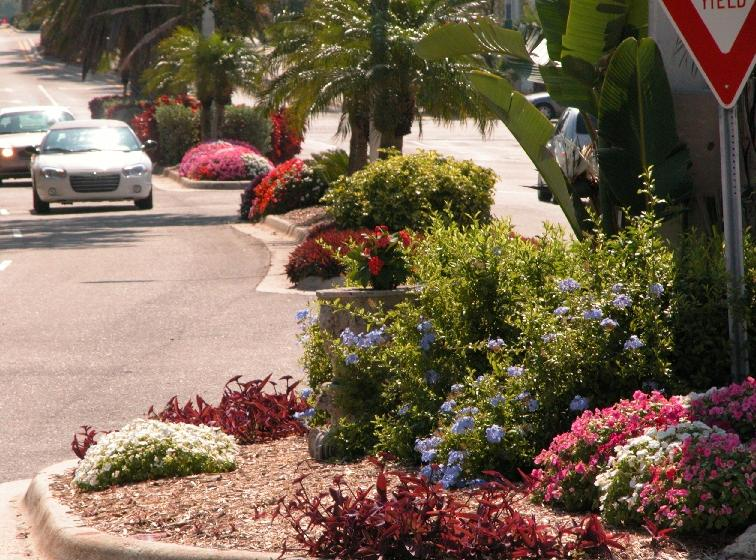
\includegraphics[width=\textwidth]{../imData/540/4.jpg}
		\caption{Original image}
	\end{subfigure}
	~
	\begin{subfigure}[b]{0.3\textwidth}
		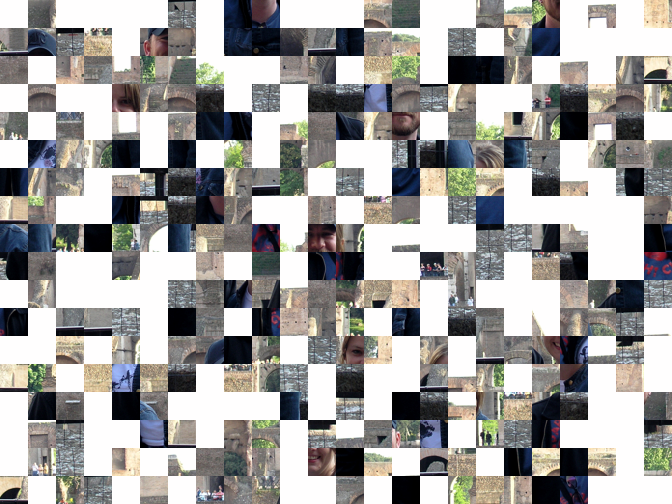
\includegraphics[width=\textwidth]{../results/540/4_shuffled.png}
		\caption{Shuffled image}
	\end{subfigure}
	~
	\begin{subfigure}[b]{0.3\textwidth}
		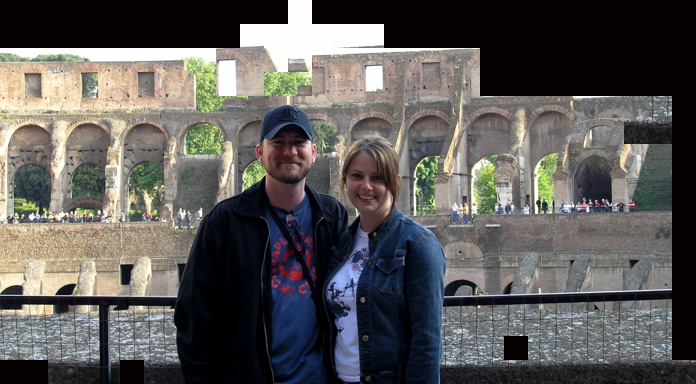
\includegraphics[width=\textwidth]{../results/540/4_solved.png}
		\caption{Solved image}
	\end{subfigure}
  ~
  \begin{subfigure}[b]{0.3\textwidth}
		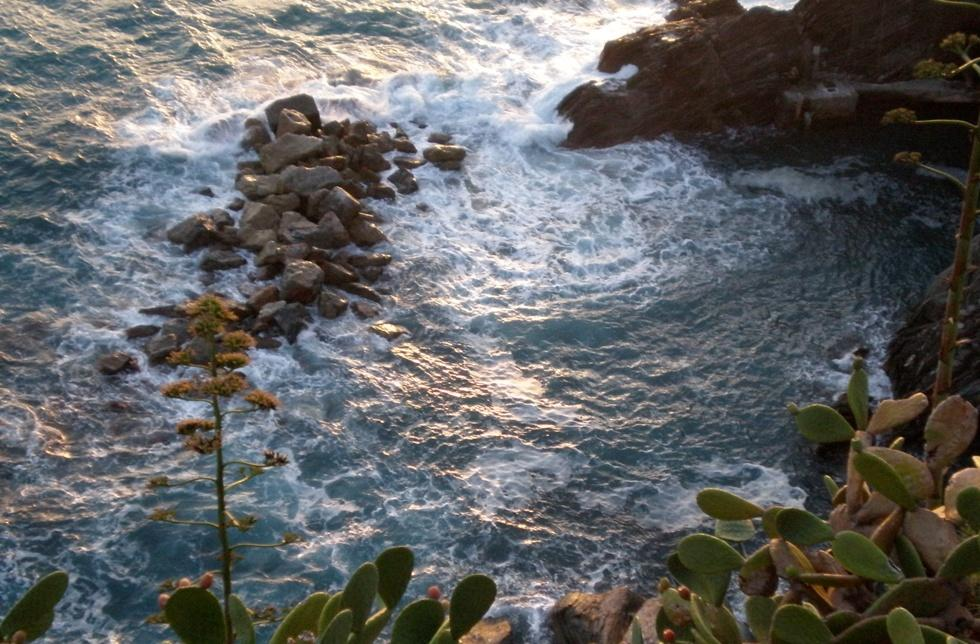
\includegraphics[width=\textwidth]{../imData/805/14.jpg}
		\caption{Original image}
	\end{subfigure}
	~
	\begin{subfigure}[b]{0.3\textwidth}
		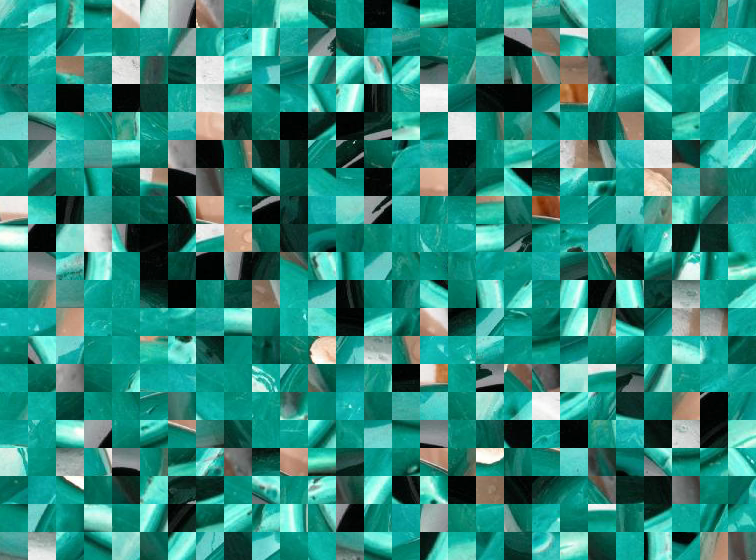
\includegraphics[width=\textwidth]{../results/805/14_shuffled.png}
		\caption{Shuffled image}
	\end{subfigure}
	~
	\begin{subfigure}[b]{0.3\textwidth}
		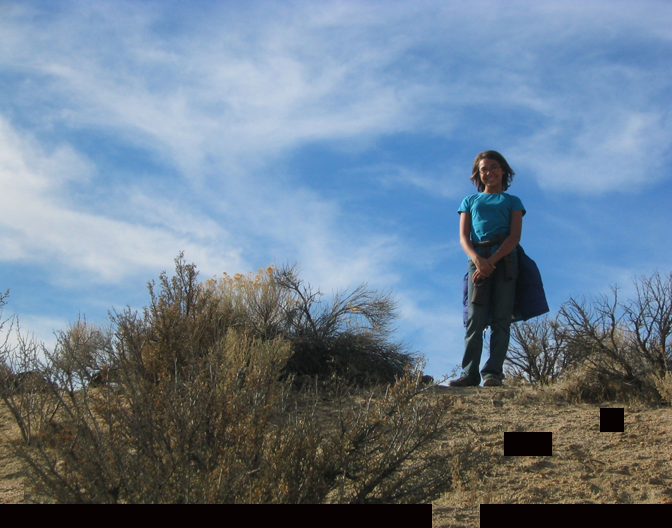
\includegraphics[width=\textwidth]{../results/805/14_solved.png}
		\caption{Solved image}
	\end{subfigure}
   ~
  \begin{subfigure}[b]{0.3\textwidth}
		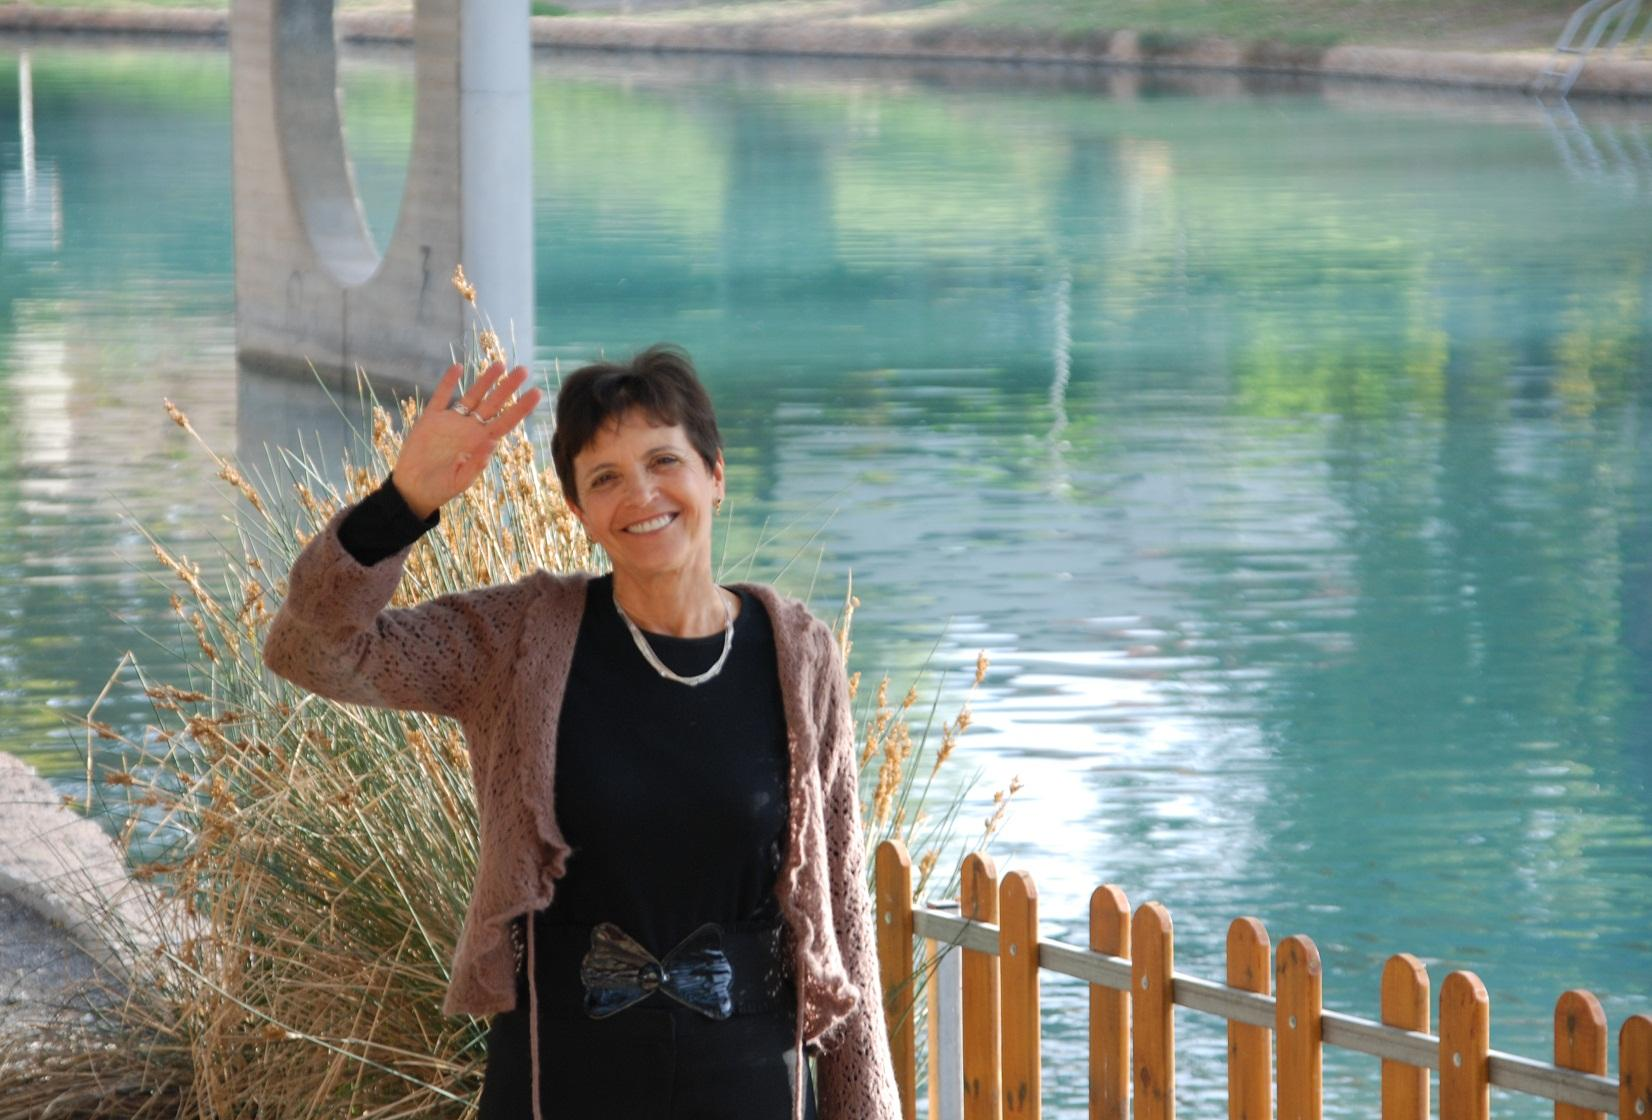
\includegraphics[width=\textwidth]{../imData/2360/1.jpg}
		\caption{Original image}
	\end{subfigure}
	~
	\begin{subfigure}[b]{0.3\textwidth}
		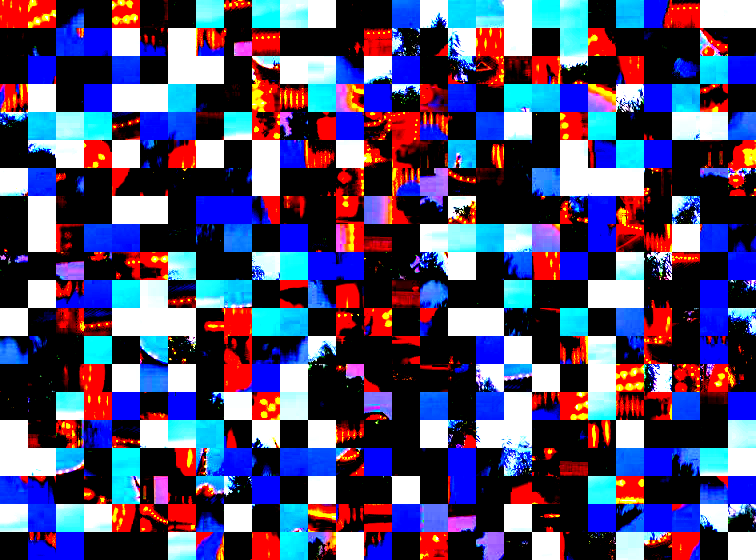
\includegraphics[width=\textwidth]{../results/2360/1_shuffled.png}
		\caption{Shuffled image}
	\end{subfigure}
	~
	\begin{subfigure}[b]{0.3\textwidth}
		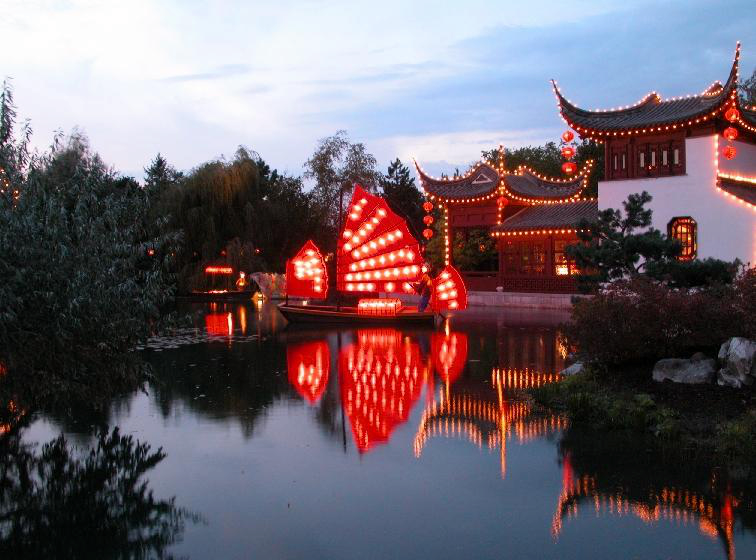
\includegraphics[width=\textwidth]{../results/2360/1_solved.png}
		\caption{Solved image}
	\end{subfigure}
	\caption{The puzzles with the highest direct measure for each puzzle size.
    Top row 432-piece puzzles, second row 540-piece puzzles, third row 805-piece
    puzzles, last row 2360-piece puzzles.}
	\label{fig:directMeasure}
\end{figure}

\begin{figure}
	\centering
	\begin{subfigure}[b]{0.3\textwidth}
		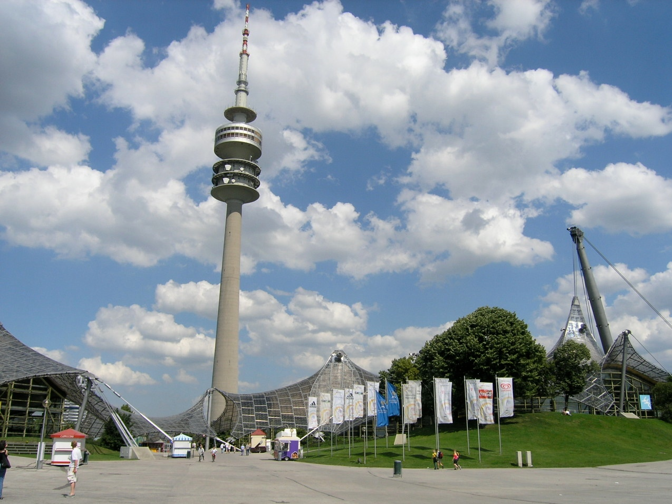
\includegraphics[width=\textwidth]{../imData/432/8.png}
		\caption{Original image}
	\end{subfigure}
	~
	\begin{subfigure}[b]{0.3\textwidth}
		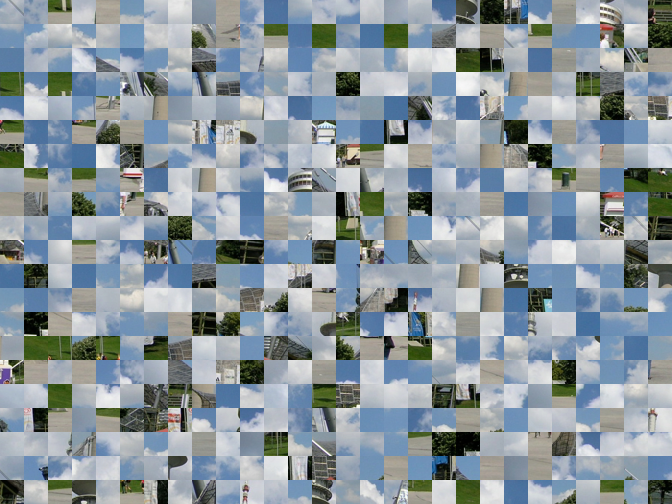
\includegraphics[width=\textwidth]{../results/432/8_shuffled.png}
		\caption{Shuffled image}
	\end{subfigure}
	~
	\begin{subfigure}[b]{0.3\textwidth}
		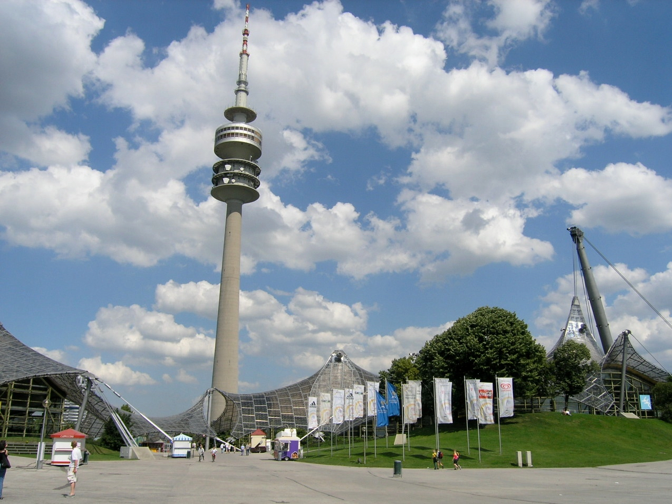
\includegraphics[width=\textwidth]{../results/432/8_solved.png}
		\caption{Solved image}
	\end{subfigure}
  ~
  \begin{subfigure}[b]{0.3\textwidth}
		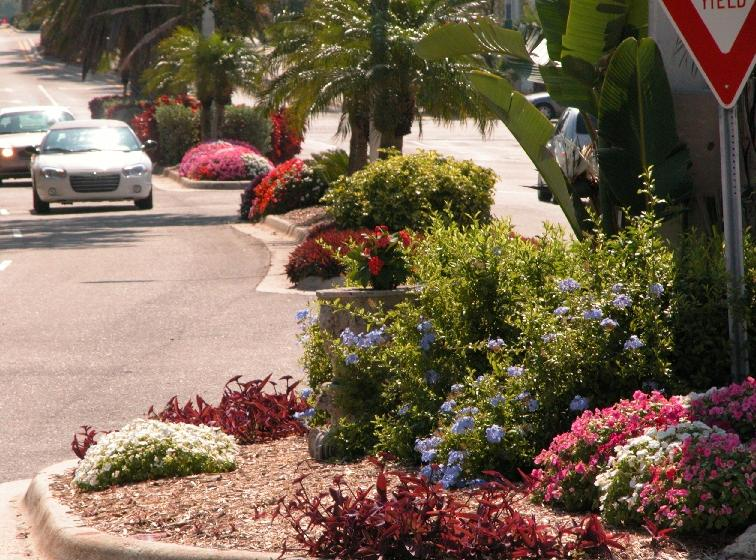
\includegraphics[width=\textwidth]{../imData/540/4.jpg}
		\caption{Original image}
	\end{subfigure}
	~
	\begin{subfigure}[b]{0.3\textwidth}
		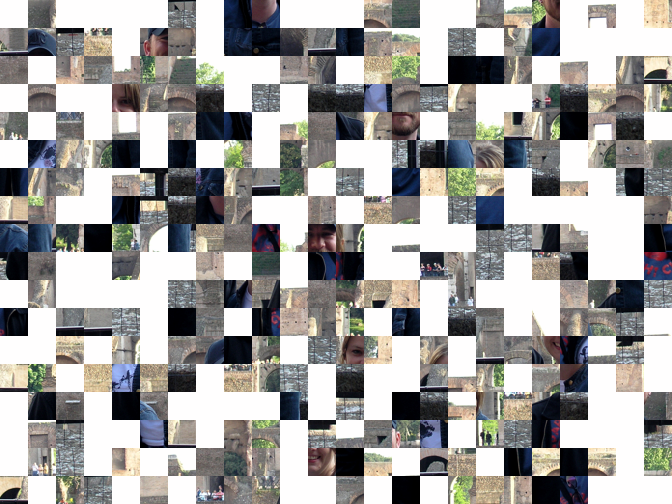
\includegraphics[width=\textwidth]{../results/540/4_shuffled.png}
		\caption{Shuffled image}
	\end{subfigure}
	~
	\begin{subfigure}[b]{0.3\textwidth}
		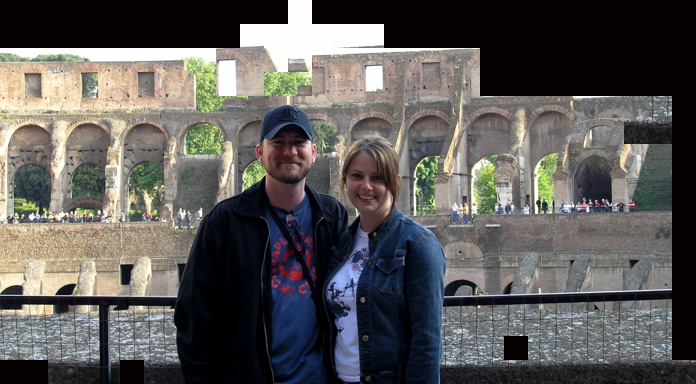
\includegraphics[width=\textwidth]{../results/540/4_solved.png}
		\caption{Solved image}
	\end{subfigure}
  ~
  \begin{subfigure}[b]{0.3\textwidth}
		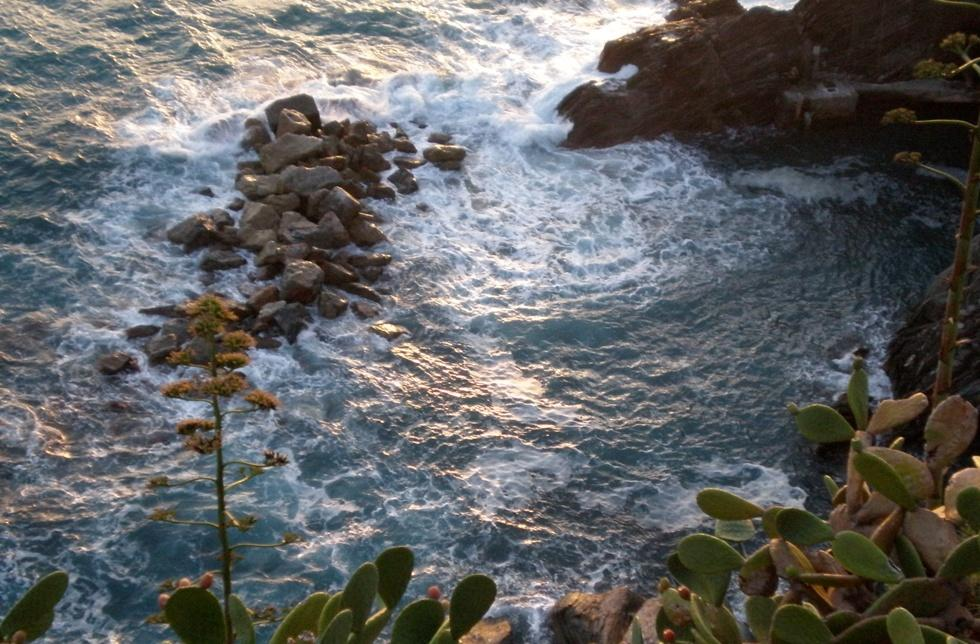
\includegraphics[width=\textwidth]{../imData/805/14.jpg}
		\caption{Original image}
	\end{subfigure}
	~
	\begin{subfigure}[b]{0.3\textwidth}
		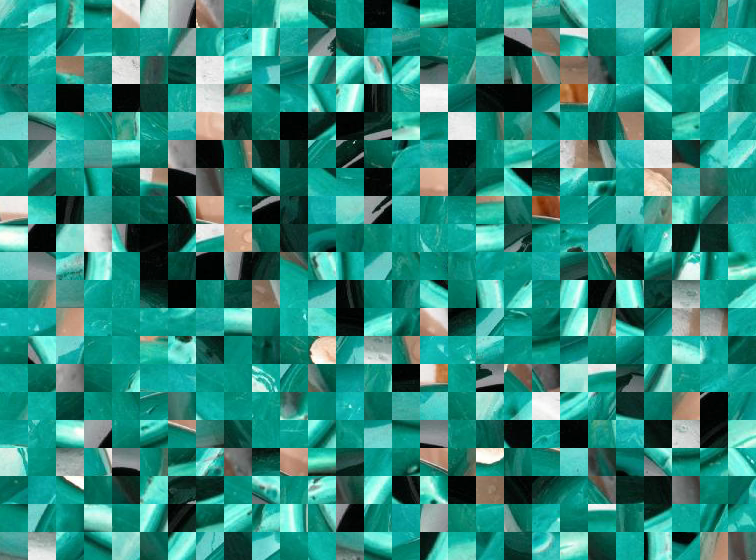
\includegraphics[width=\textwidth]{../results/805/14_shuffled.png}
		\caption{Shuffled image}
	\end{subfigure}
	~
	\begin{subfigure}[b]{0.3\textwidth}
		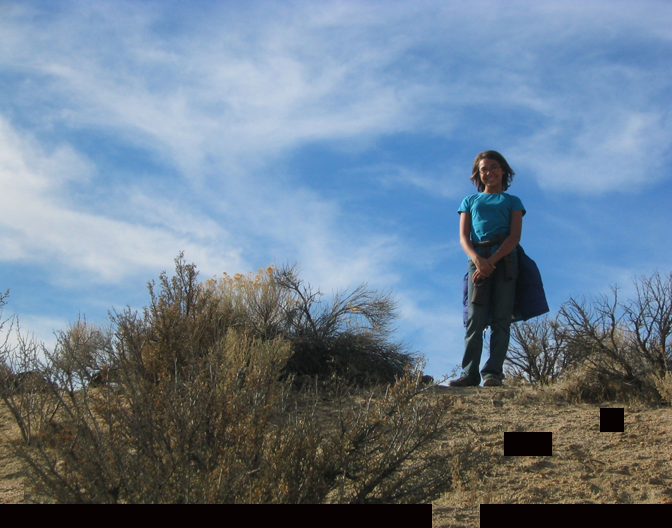
\includegraphics[width=\textwidth]{../results/805/14_solved.png}
		\caption{Solved image}
	\end{subfigure}
   ~
  \begin{subfigure}[b]{0.3\textwidth}
		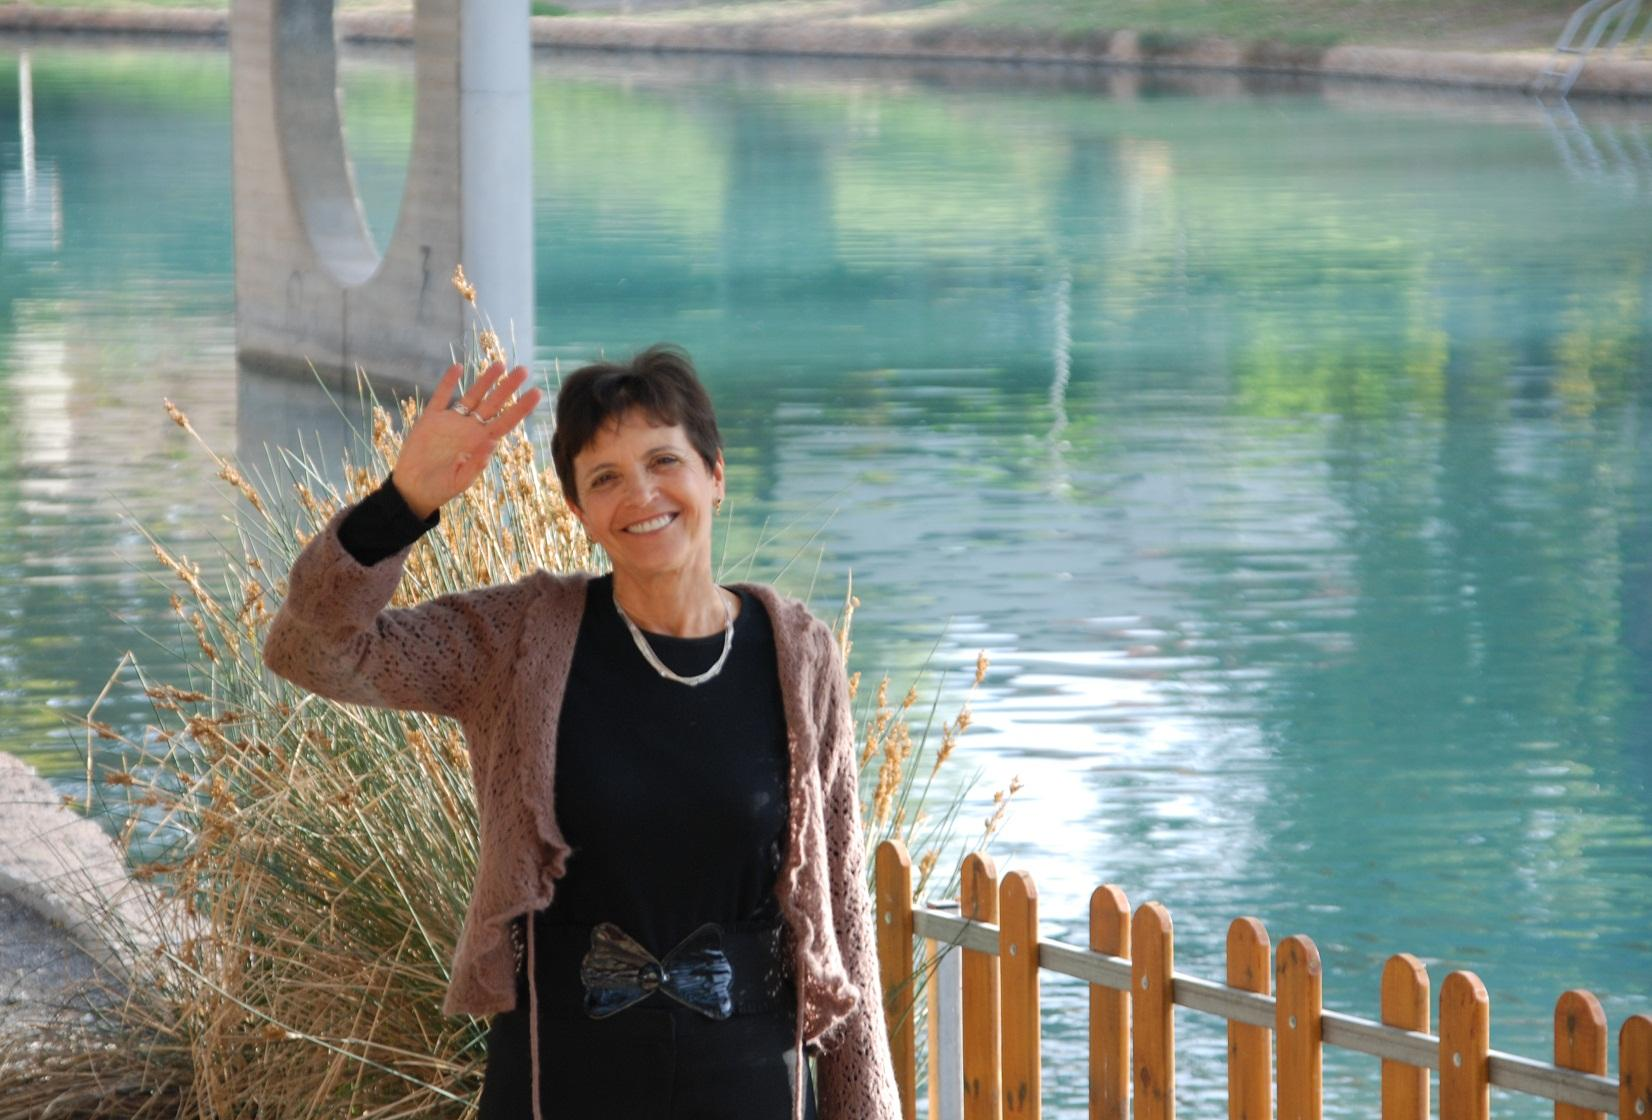
\includegraphics[width=\textwidth]{../imData/2360/1.jpg}
		\caption{Original image}
	\end{subfigure}
	~
	\begin{subfigure}[b]{0.3\textwidth}
		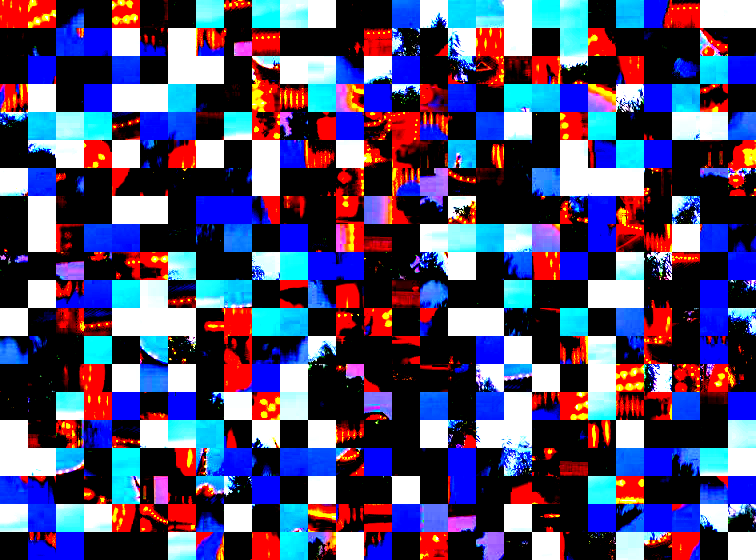
\includegraphics[width=\textwidth]{../results/2360/1_shuffled.png}
		\caption{Shuffled image}
	\end{subfigure}
	~
	\begin{subfigure}[b]{0.3\textwidth}
		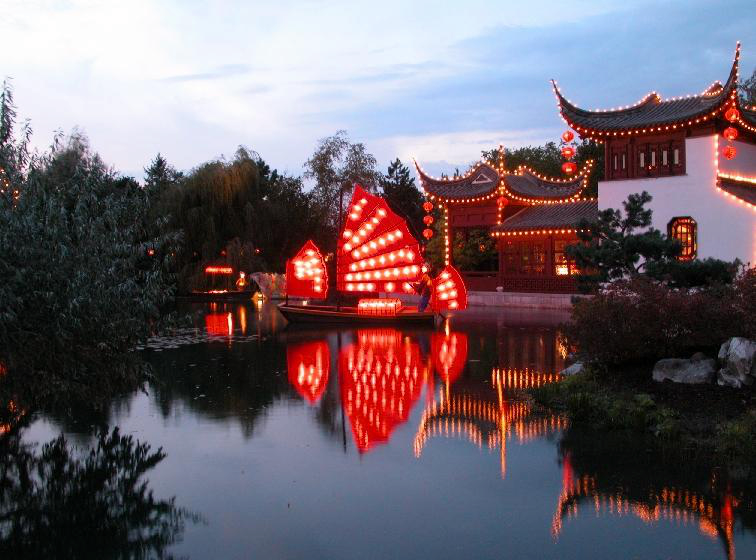
\includegraphics[width=\textwidth]{../results/2360/1_solved.png}
		\caption{Solved image}
	\end{subfigure}
	\caption{The puzzles with the highest neighbor measure for each puzzle size.
    Top row 432-piece puzzles, second row 540-piece puzzles, third row 805-piece
    puzzles, last row 2360-piece puzzles.}
	\label{fig:neighborMeasure}
\end{figure}



\bibliography{literature}

\end{document}    
